% !TeX root = vpl.tex

\chap{The Robot Finds Its Way by Itself}\label{ch.line}

Consider a warehouse with robotic carts that bring objects to a central
dispatching area. There are lines painted on the floor of the warehouse
and the robot receives instructions to follow certain lines until it
reaches the storage bin of the desired object. Let us write a program
that causes the robot to follow a line on the floor.

{\raggedleft \hfill Program file \bu{follow-line.aesl}}

The line-following task brings out all the uncertainty of constructing
robots in the real world: The robot must deal with uncertainty in its
perceptions and its actions. For instance, the line might not be
perfectly straight, dust may obscure part of the line, or dirt may cause
one wheel to move more slowly than the other one. To follow a line, the
robot must use a \emph{controller} that decides how much power to apply
to each motor depending on the data received from the sensors.

\sect{The line and the robot}

To follow a line, we use the ground sensors (\cref{ch.moving}). Remember
that these work by sending infrared light (which is invisible to human
eye) and measuring how much is reflected back. If the floor is
light-colored, the sensor will detect a lot of reflected light and the
event \blksm{lots-of-light} will occur. We need a line that will cause
an event to occur when there is little reflected light
\blksm{little-light}. This is easy to do by printing a black line on
paper and taping it to the floor, by painting the line, or by sticking
black electrician's tape on the floor (\cref{fig.tape}). The line must
be wide enough so that both ground sensors will sense black when the
robot is successfully following the line. A width of 5 centimeters is
sufficient for the robot to follow the line even if there are small
deviations.

\begin{figure}
\subfigure[Thymio following a line of tape]%
{\label{fig.tape}%
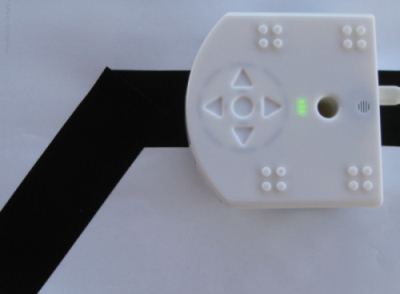
\includegraphics[height=0.35\textwidth]{blacktape}}
\hfill
\subfigure[The left sensor is off the tape and the right sensor is on the tape]%
{\label{fig.one-off}%
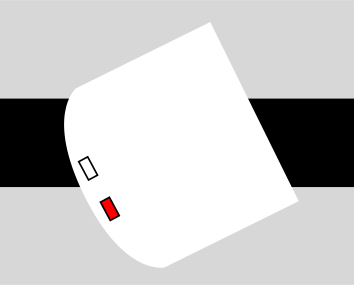
\includegraphics[height=0.35\textwidth]{thymio_half_on_line}}
\caption{Thymio on a black tape}
\end{figure}

To implement line-following, first, we cause the robot to move forward
whenever \emph{both} sensors detect a dark surface (it is on the line)
and to stop whenever \emph{both} sensors detect a light surface (it is
not the line):

The event-actions pairs are shown in \cref{fig.start-stop}.
                  
\begin{figure}
\subfigure[Start and stop the robot]%
{\label{fig.start-stop}%
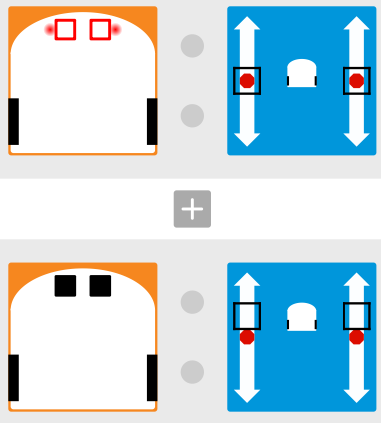
\includegraphics[width=0.4\textwidth]{line-forward}}
\hfill
\subfigure[Correcting deviations]%
{\label{fig.follow-line}%
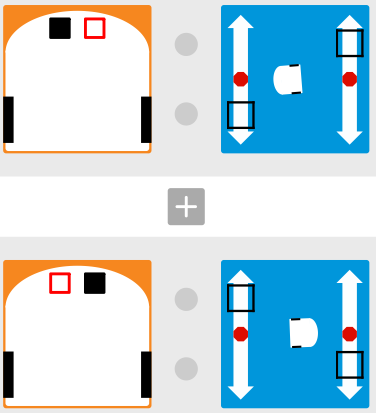
\includegraphics[width=0.4\textwidth]{line-controller}}
\caption{A program for line following}
\end{figure}

%\begin{center}
%\begin{tabular}{cc}
%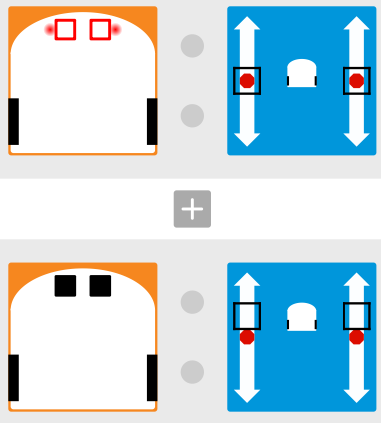
\includegraphics[width=0.4\textwidth]{line-forward} &
%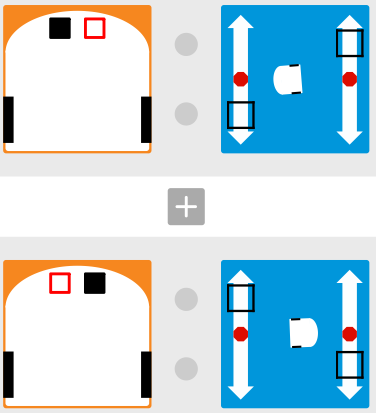
\includegraphics[width=0.4\textwidth]{line-controller} \\
%(a) Start and stop the robot & (b) Follow the line \\
%\end{tabular}
%\end{center}

\trickbox{Make sure that you use a USB cable that is long enough (say,
two meters), so that the Thymio can stay connected to the computer even
as it moves. You can find extension cables in any computer shop.}

\sect{Your first controller}

The next step is to program the controller that follows the line. Two
event-actions pairs are needed, as shown on the image above (b):

\begin{itemize}

\item If the robot moves off the tape to the \emph{left}
(\cref{fig.one-off}), the \emph{left} sensor will detect the floor while
the \emph{right} sensor is still detecting the tape; in that case the
robot should turn slightly to the \emph{right}.

\item If the robot moves off the tape to the \emph{right}, the
\emph{right} sensor will detect the floor while the \emph{left} sensor
is still detecting the tape; in that case the robot should turn slightly
to the \emph{left}.

\end{itemize}

%Two event-actions pairs are needed, as shown in \cref{fig.follow-line}.

\sect{Setting the parameters}

It is easy to see that if the robot runs off the left edge of the tape,
it has to turn to the right (\cref{fig.one-off}). The question is
how tight should the turn be? If the turn is too gentle, the right
sensor might \emph{also} run off the tape before the robot turns back;
if the turn is too aggressive, it might cause the robot to run off the
other end of the tape. In any case, aggressive turns can be dangerous to
the robot and whatever it is carrying.

You will need to experiment with the speeds of the left and right motors
in each motor action block until the robot runs \emph{reliably}. Here,
reliably means that the robot can successfully follow the line several
times. Since each time you place the robot on the line you might place
it at a slightly different position and point in a slightly different
direction, you need to run several tests to make sure that the program
works.

There are many ways to configure the motor action blocks. The forward
speed of the robot on the line is an important parameter. If it is too
fast, the robot can run off the line before the turning actions can
affect its direction. However, if the speed is too slow, no one will buy
your robot to use in a warehouse.

If the robot starts to leave the line, what should it do? If it makes a
sharp turn (one motor goes forward and the other backwards), the robot
will return quickly to the line, but its movements will be very jerky.
On the other hand, if the robot makes a gentle turn (one motor goes
slightly faster than the other), the robot will move smoothly but it may
lose the line. You will have to experiment to find good compromises.

\newpage

\exercisebox{\thechapter.1}{The robot stops when both ground sensors
detect that they are off the tape. Modify the program so that the robot
makes a gentle left turn in an attempt to find the tape again. Try it on
a tape with a left turn like the one shown in \cref{fig.tape}. Try
increasing the forward speed of the robot. What happens when the robot
gets to the end of the tape?}

\bigskip

\exercisebox{\thechapter.2}{Modify the program from the previous
exercise so that the robot turns right when it runs off the tape. What
happens?
\vspace{.5em}\\
It would be nice if we could \emph{remember} which sensor was the last
one to lose contact with the tape in order to cause the robot turn in
the correct direction to find the tape again. In \cref{ch.states} we
will learn how Thymio can remember information.}

\bigskip

\exercisebox{\thechapter.3}{
Experiment with different arrangements of the lines of tapes:
\begin{itemize}[noitemsep,nosep,leftmargin=*]
\item Gentle turns;
\item Sharp turns;
\item Zigzagging lines;
\item Wider lines;
\item Narrow lines.
\end{itemize}
Run competitions with your friends: Whose robot successfully follows the
most lines? For each line, whose robot follows it in the shortest time?
}

\bigskip

\exercisebox{\thechapter.4}{
Discuss what effect the following modifications to the Thymio would
have on the ability of the robot to follow a line:
\begin{itemize}[noitemsep,nosep,leftmargin=*]
\item Ground sensing events occur more often or less often than 10 times a second;
\item The sensors are further apart or closer together;
\item There are more than two ground sensors on the bottom of the robot.
\end{itemize}
}
